\chapter{Semantic Description of Road Systems}
\label{ch:descriptionOfRoadSystems}
The following chapter provides a thorough description of the models and semantic description generation process for an urban aria from ESRI CityEngine (CE) using data provided by OpenStreetMap (OSM). Moreover, we provide a detailed explanation of the resulting JSON format which holds information about essential scene data. Lastly, we explain how the resulting file is parsed and used by Unity3D. Additionally, we defend design decisions, as well as describe failed attempts in the process.

A general overview of the whole process can be seen in Figure \ref{fig:overview}. Firstly, OSM data of a given area is sanitised and imported in CE. The same sanitised data is provided to SUMO, which generates additional road details which are not present in CE. Afterwards, 3D models are generated together with the combined from CE and SUMO semantic road description. In the end, they are imported and utilised in Unity3D. The navigation module which can be seen in \emph{Unity Game Engine} will be discussed in Chapter \ref{ch:gps}.

\begin{figure}[htb]
	\centering
	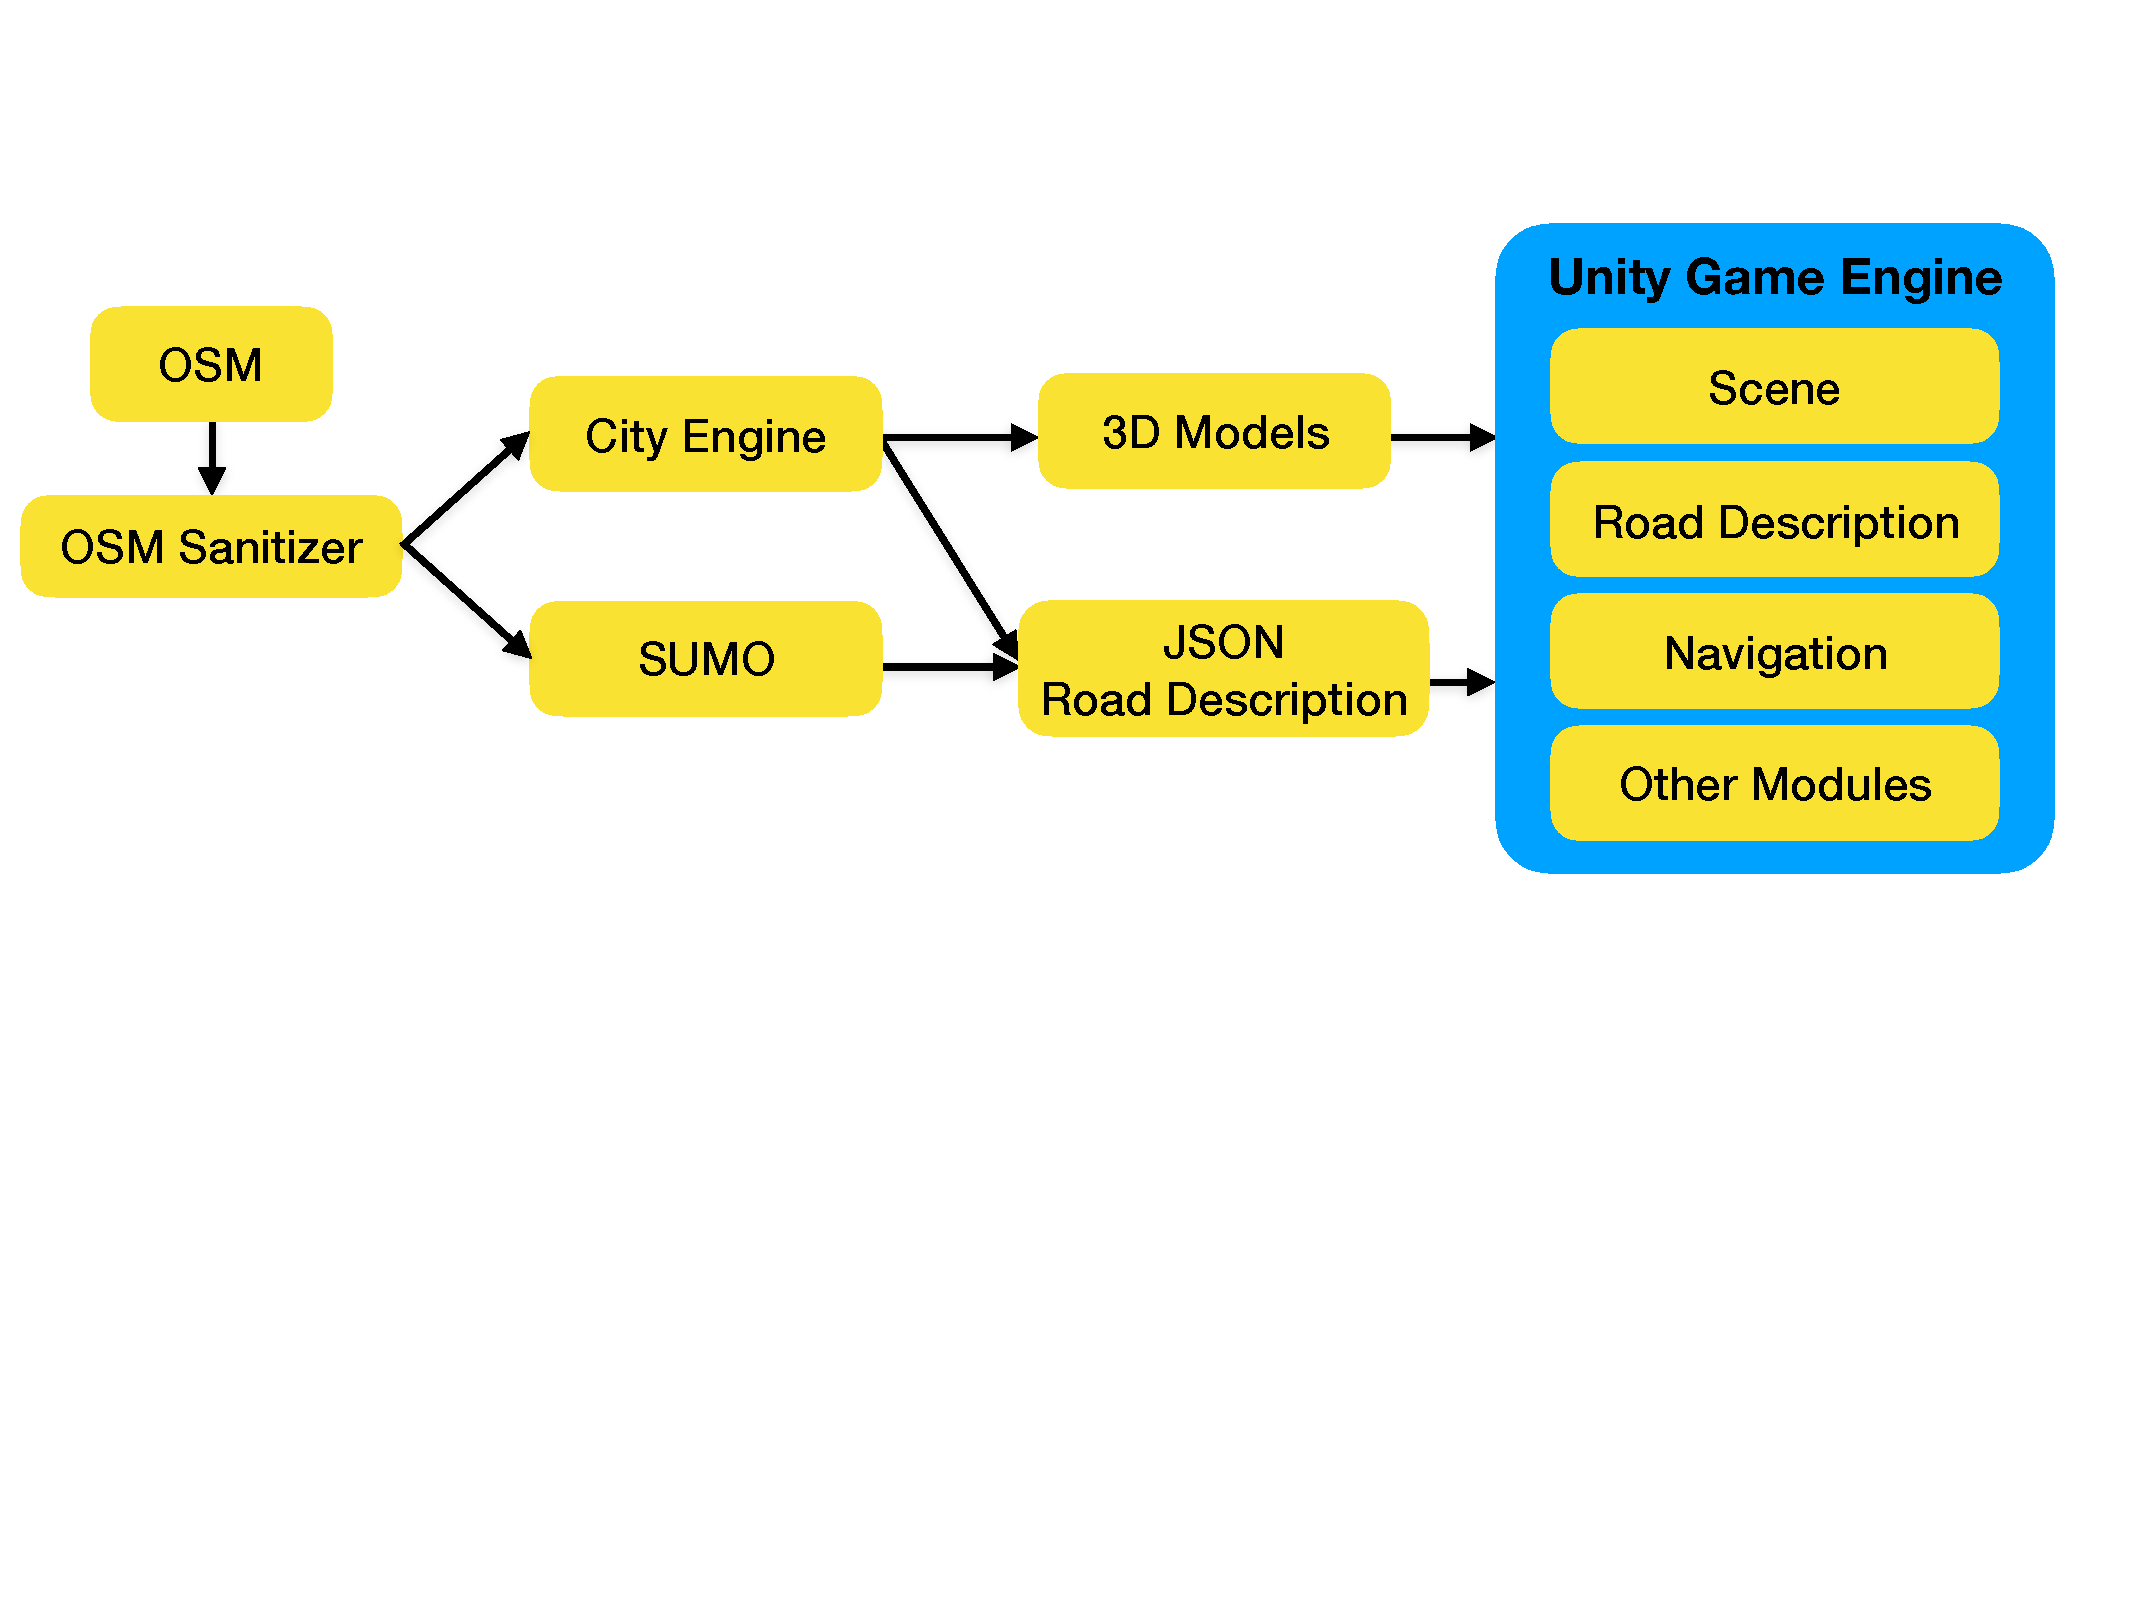
\includegraphics[width=0.95\linewidth]{figures/overview}
	\caption{Overview of the scene creation workflow.}
	\label{fig:overview}
\end{figure}

\section{OSM Export}
As already introduced, the whole map data used in the MMK Driving Simulator is exported from OSM. In Figure \ref{fig:overview} we can see that exported \emph{OSM} file is fed to a \emph{OSM Sanitizer}. There are multiple reasons why this is necessary. Firstly, the objects contained in the export include some unnecessary information which are not present in the simulation, \emph{e.g.} underground network, footpaths. Moreover, this additional objects in the map represent a obstacle for both SUMO and CE when they are building a scene. For example, in Figure \ref{fig:nosimply} and \ref{fig:simply} one could see the difference in the shape creation between respectively a unsanitised and sanitised version of the same \emph{OSM} export data.  

\begin{figure}[htb]
	\centering
	\subfigure[Unsanitised] {
	  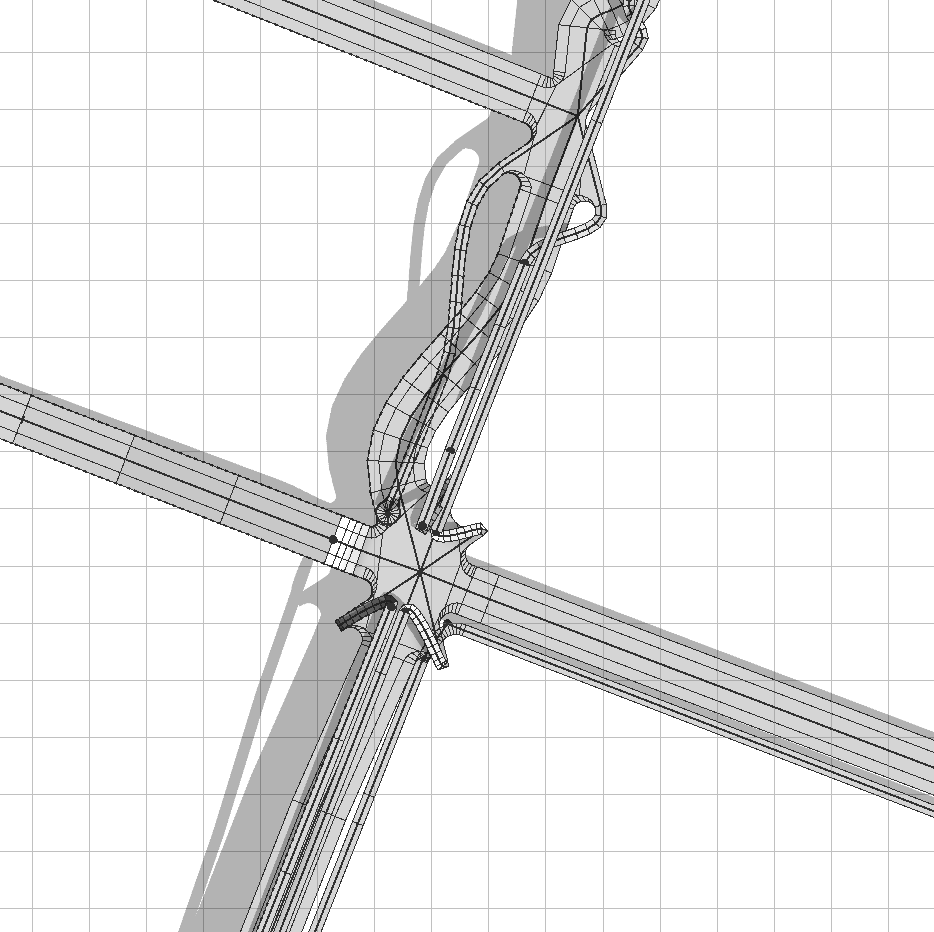
\includegraphics[width=0.4\textwidth]{figures/no-simply}
	  \label{fig:nosimply}
	}\hspace{0.05\textwidth}% \hfill or \hspace{5mm} or \hspace{0.3\textwidth}
	\subfigure[Sanitised] {
	  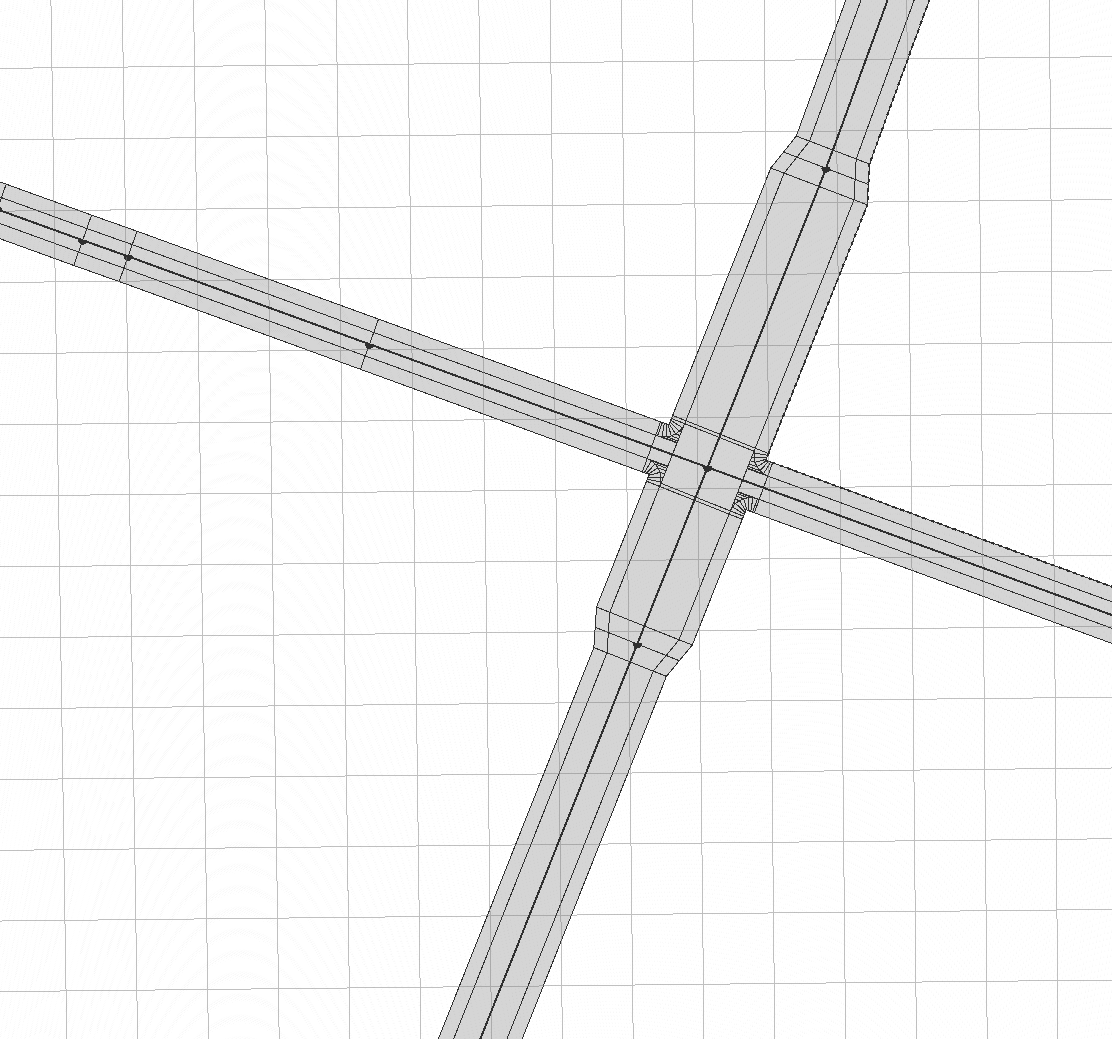
\includegraphics[width=0.4\textwidth]{figures/simply}
	  \label{fig:simply}
	}
	\caption{Comparison of the same CityEngine generated shapes from unsanitised and sanitised \emph{OSM} export file.}
\end{figure}

Since the information in the OSM export is only 2D, CE attempts to to find the perfect location for every shape, although most of them overlap. Therefore, it chooses \texttt{y} values which would generate reasonable shapes. Clearly, the scene generated in this way could not be used in Unity, so we have to delete some of the data. This was achieved by a Python3 script which can be found in \texttt{cityengine-mmk/scripts/osmsanitizer.py}. The script accepts only one input parameter, which is the OSM export file and produces a sanitised version of the same export with the appendix \texttt{-sanitized} in its name. The script can be executed in the console as follows assuming we are in the same folder as the script: \texttt{python3 osmsanitizer.py ../data/map.osm}. The result \texttt{map-sanitized.osm} will be again situated in \texttt{cityengine-mmk/data} folder. 

The sanitisation process follows a straightforward whitelisting fashion. Firstly, we have to delete all roads which are not drivable by a vehicle. Additionally, we want to preserve information about buildings and parkings which should be also present in the export. As we know from Chapter \ref{ch:background}, there are two main objects in OSM which hold information about the infrastructure of the road network: \texttt{way} and \texttt{relation}. According to the OSM documentation\footnote{\url{http://wiki.openstreetmap.org/wiki/Key:highway}}, all streets (\texttt{way} objects) must have a \texttt{highway} tag which marks its type. The valid highway tags are \texttt{motorway}, \texttt{motorway\_link}, \texttt{trunk}, \texttt{trunk\_link}, \texttt{primary}, \texttt{primary\_link}, \texttt{secondary}, \texttt{secondary\_link}, \texttt{tertiary}, \texttt{tertiary\_link}, \texttt{unclassified}, \texttt{residential}, \texttt{living\_street}, \texttt{unsurfaced}. If a \texttt{way} object does not contain a \texttt{highway} tag or the type of the road is not one of the aforementioned fourteen values, then it is deleted. Similarly, we check whether a \texttt{way} object contains a \texttt{building} tag which is set to \texttt{yes} and a \texttt{amenity} tag set to \texttt{parking}. This approach leaves in the OSM export buildings and parkings which coordinates and properties can be later imported in CE.

The sanitiser tries to solve another problem with OSM data, too. Sometimes information about streets, \emph{e.g.} maximum allowed speed or number of lanes, could be missing. When this is the case CE and SUMO try to extrapolate this information and suggest some valid values in order to create the resulting 3D models. Unfortunately, it could happen that both softwares provide different values for the same segment. Because we want to integrate the information streams coming from both, CE and SUMO to create a semantic description of the road network, this data extrapolation has to accomplished one step ahead in the sanitisation process. Therefore, we provide default valid values for missing information and add it to the OSM objects in the final sanitised file.

Finally, we have an OSM data which is valid and contains only the necessary information to build 3D shapes from it. Note that we do not delete any \texttt{node} objects because unused nodes, \emph{i.e.} not connected by a way or a relationship, are by default discarded in both, CE and SUMO.

\section{Semantic Description}
After we have accomplished the sanitisation of the OSM data, we can feed the resulting file to both CityEngine and SUMO as can be seen in Figure \ref{fig:overview}. Overall, we use the CE's Python interface to traverse all necessary objects and extract their properties. Afterwards, using the OSM ID, we extract lane information about the road network generated by SUMO, which is not available in CE. In the end, the combined information from CE and SUMO is exported as JSON format, which structure is described in Section \ref{sec:format}. 

\subsection{OSM Data Import Process}
In order to build a 3D urban scene accompanied by a semantic description of the road system, the user has to execute the steps which will be described in this section. Some of the steps were not able to be automated because of limitations related to CE. After starting a CE instance and opened the \texttt{cityengine-mmk} project which contains some essential rules to generate the 3D models, the user have to create a new empty scene. The sanitised OSM file has to be in \texttt{cityengine-mmk$\backslash$data} folder. Now the user can drag the file to the 3D viewport and a similar window as in Figure \ref{fig:import} will show up. Since we have removed all of the unnecessary object from the OSM file, we have just select all properties to be imported. Next, we can leave the \emph{Map OSM tags} selected, because we will need them later in the export process. Although our sanitiser has prepared the data, we still need \emph{Run Graph Cleanup Tool after Import} option because sometimes OSM data can be still imprecise. This option will delete unnecessary nodes and segments which overlap each other or are incomplete. Finally, we want CE to generate shapes for the road network, therefore we mark the \emph{Create Street/Intersection Shapes from Graph} option, too. There is a way to import an OSM map data directly using the CE's Python interface using \texttt{CE.importFile} and \texttt{OSMImportSettings}. Unfortunately, there is no way to select which of the each object's attributes to be imported. Moreover, only some of the attributes are selected by default which is not sufficient for our purposes. In the end, one have to select \emph{Finish} and the software will import the data and generate 3D shapes. An example import of the \emph{TU Viertel} in M\"unchen\footnote{\url{https://www.openstreetmap.org/#map=16/48.1493/11.5678}} can be seen in Figure \ref{fig:ce-1}.

\begin{figure}[htb]
	\centering
	\subfigure[] {
	  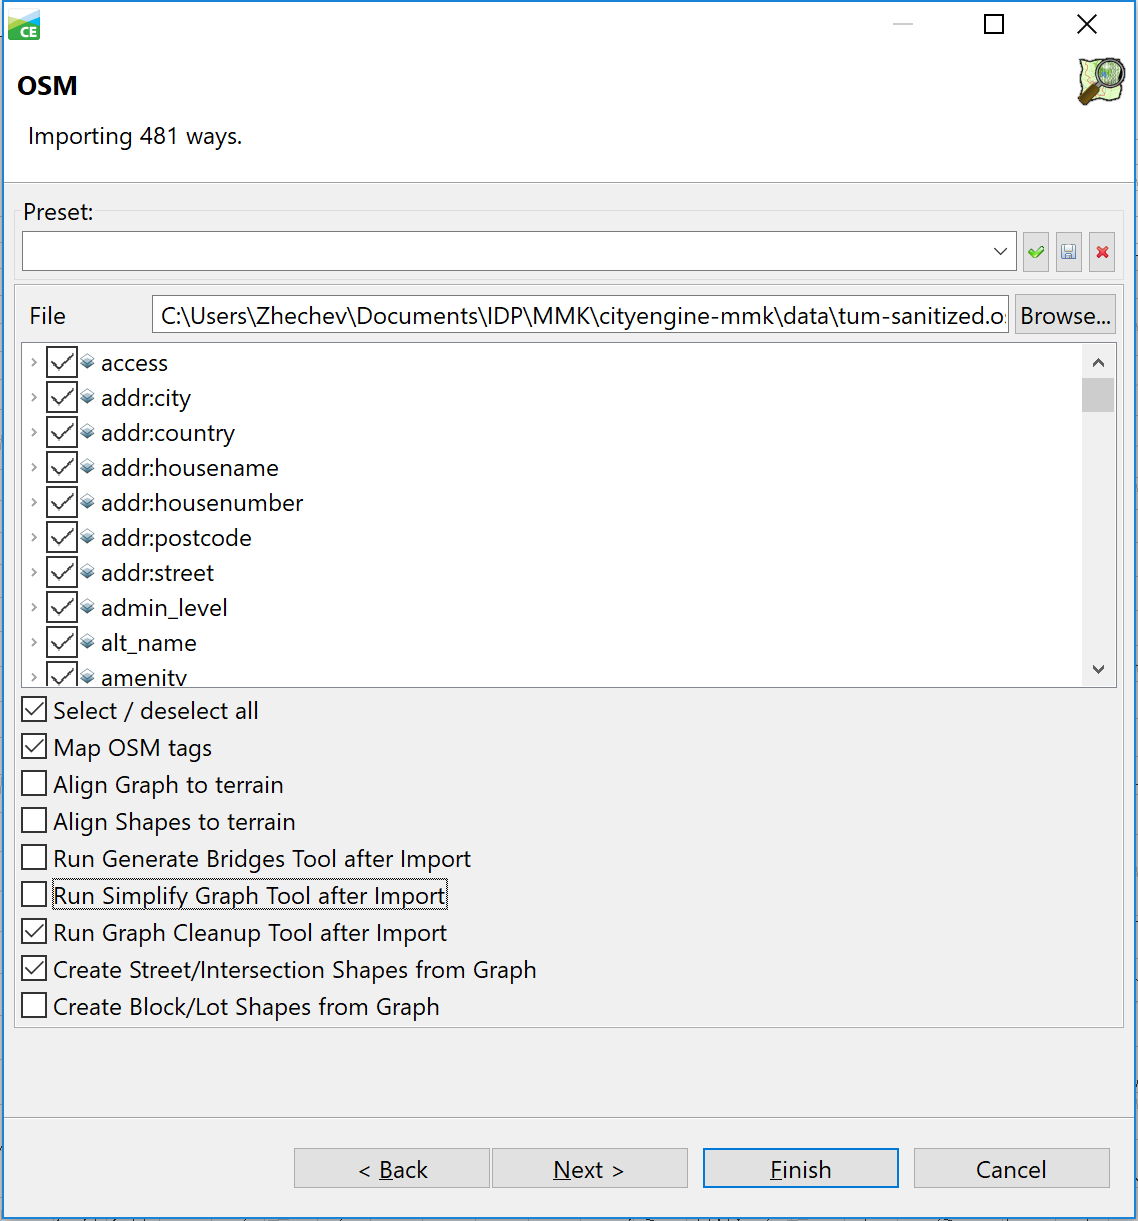
\includegraphics[width=0.28\textwidth]{figures/import}
	  \label{fig:import}
	}%\hspace{0.05\textwidth}% \hfill or \hspace{5mm} or \hspace{0.3\textwidth}
	\subfigure[] {
	  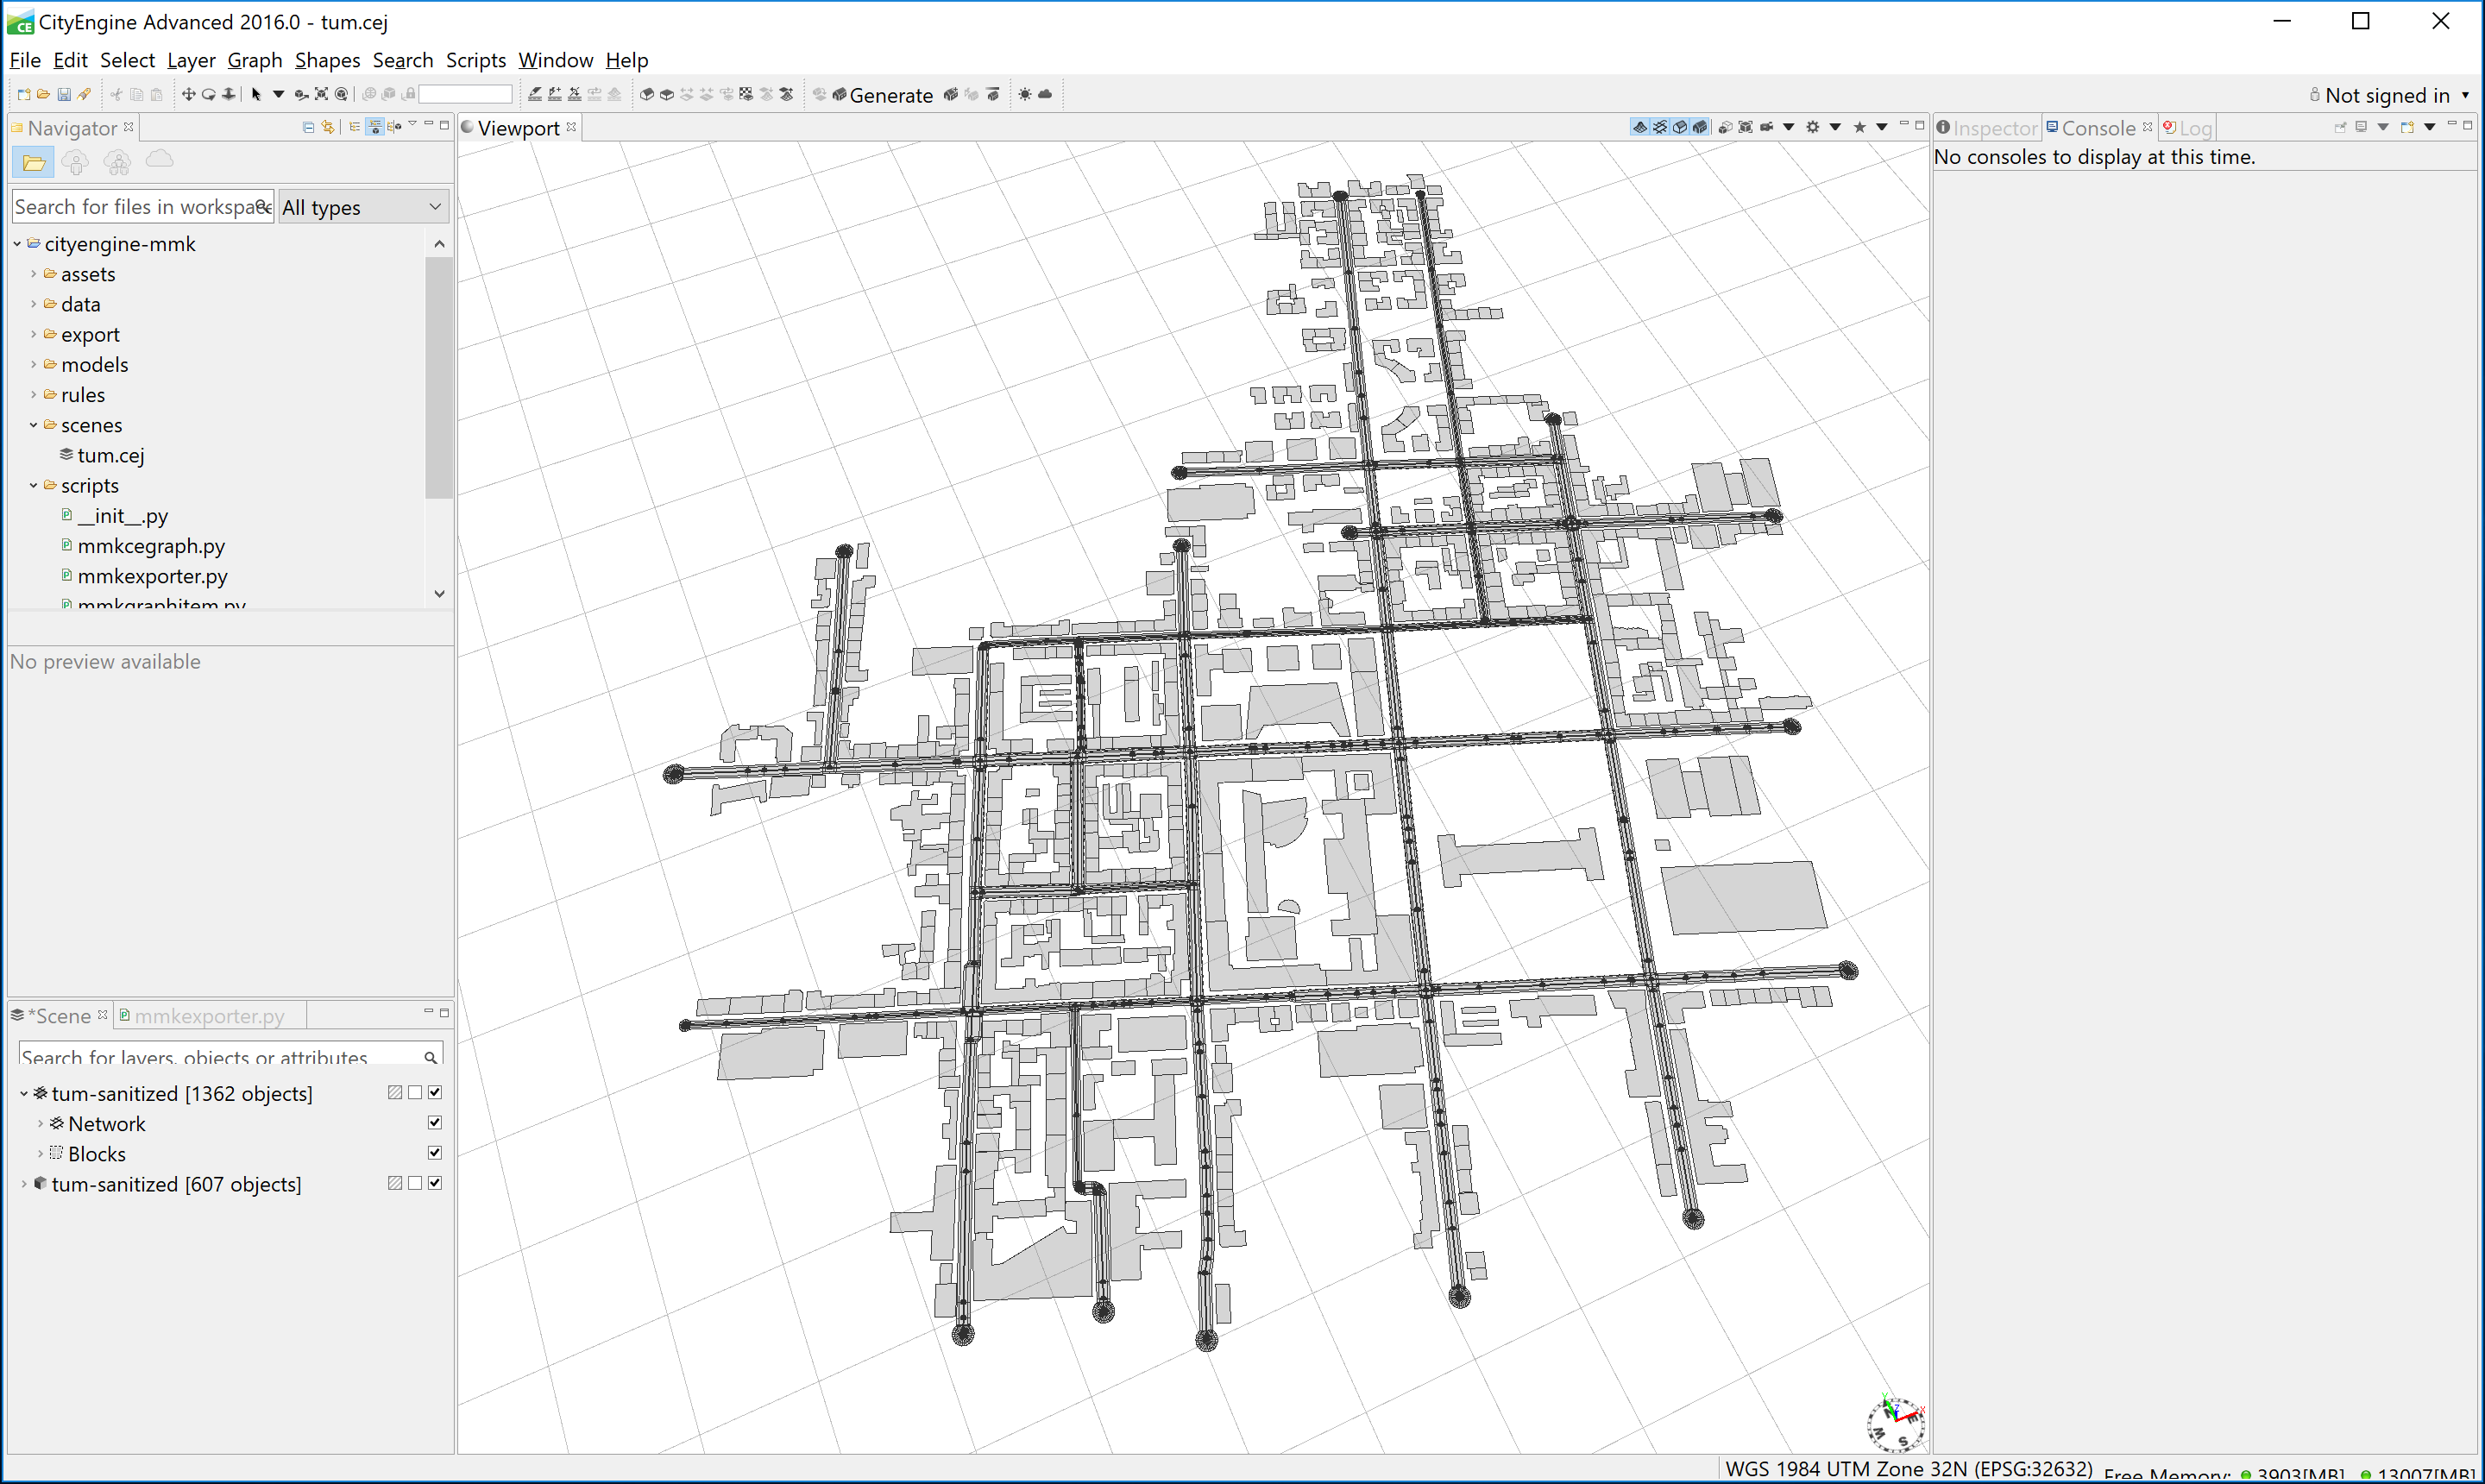
\includegraphics[width=0.68\textwidth]{figures/ce-1}
	  \label{fig:ce-1}
	}
	\caption{Example import dialog of OSM data in CE (a) and the resulting scene (b).}
\end{figure}

\subsection{CE Settings and Way-Segment Inconsistencies}
If we happen to leave the \emph{Run Simplify Graph Tool after Import} option marked, it may alter the imported OSM information, thus making it useless for cross referencing data between OSM and CE. The simplifying strategy of CE tries to merge some neighbouring segments in order to make the underlying road system more straight. Unfortunately, the CE's algorithm tries to merge properties of segments which are not meant to be combined. If it happens that the two segments, which are going to be combined, posses different OSM ID values, then the new segment receives the arithmetic mean of the two values. Of course, this new ID is not value and we cannot restore the original segments' IDs which renders it ineffective. To face this problem, we selected separately segments which have the same OSM IDs and called the simplifying tool only for them. Fortunately, this solved the problem with the destroyed IDs, nonetheless it broke junction's connections. In that case, two ways which were crossing in the middle forming a junction, were separated by CE in 4 segments, one for each exit of the junction. Calling the simplifying tool separately for the two pairs deleted the junction and placed one of the roads above the other. Clearly, this was not a solution to this problem, so we decided to unmark this tool since all of the generated shapes until this moment were acceptable.  

Another setting which could alter the shape generation process in a negative way and therefore decrease the reality of the produced scene is \emph{Run Generate Bridges Tool after Import}. This tool determines whether a segment's \texttt{y} value can be changed so it is lifted above another, underlying structure. This approach introduces some inaccuracies in the generated road models. Since this tool is absent from SUMO (it is only a 2D simulation) and we have to keep the shapes of the two generated urban networks as close as possible, we chose to switch off this option. However, this also means that the user have to furthermore adjust the shapes of some objects to represent the reality while staying coherent to SUMO.

Our first approach to create a semantic description of the road network in CE generated using OSM data involves completely ignoring the imported parameters in CE. We still have to export the vertices related to the CE's shapes using the CE's Python interface but all of the information about a given street segment such as number of lanes or speed limits will be directly taken from the OSM export file. The biggest advantage of this approach is that we can accomplish the \texttt{xml}-parsing in Python 3 which might be more performant than using the Jython interface in CE to read all of the attributes. Although this is generally true, we would break the export functionality in two big modules which are highly coherent and belong in one place. Moreover, there was another obstacle which seemed crucial for the success of this approach. CE does place almost (actually this causes yet another problem which will be discussed later in this section) every OSM node on its correct place and uses its original OSM ID, but this is not the case with segments. According to the shape of a given way (which is determined by its nodes), CE decides in how many actual segments to partition it. In other words, it may happen that one \texttt{way} object has more than one corresponding segments in the CE scene. Unfortunately, this introduces unnecessary difficulties in reconstructing a way from its segments which would be later crucial for the lane generation. Therefore, this first approach was abandoned in favour of a script purely implemented in the CE's Jython environment which depends on the imported attributes in CE from OSM to reconstruct each object's behaviour. 

\subsection{CE Export}
	Explain the whole CE export without lanes including translation\\
	Implementation details - UML

\begin{figure}[htb]
	\centering
	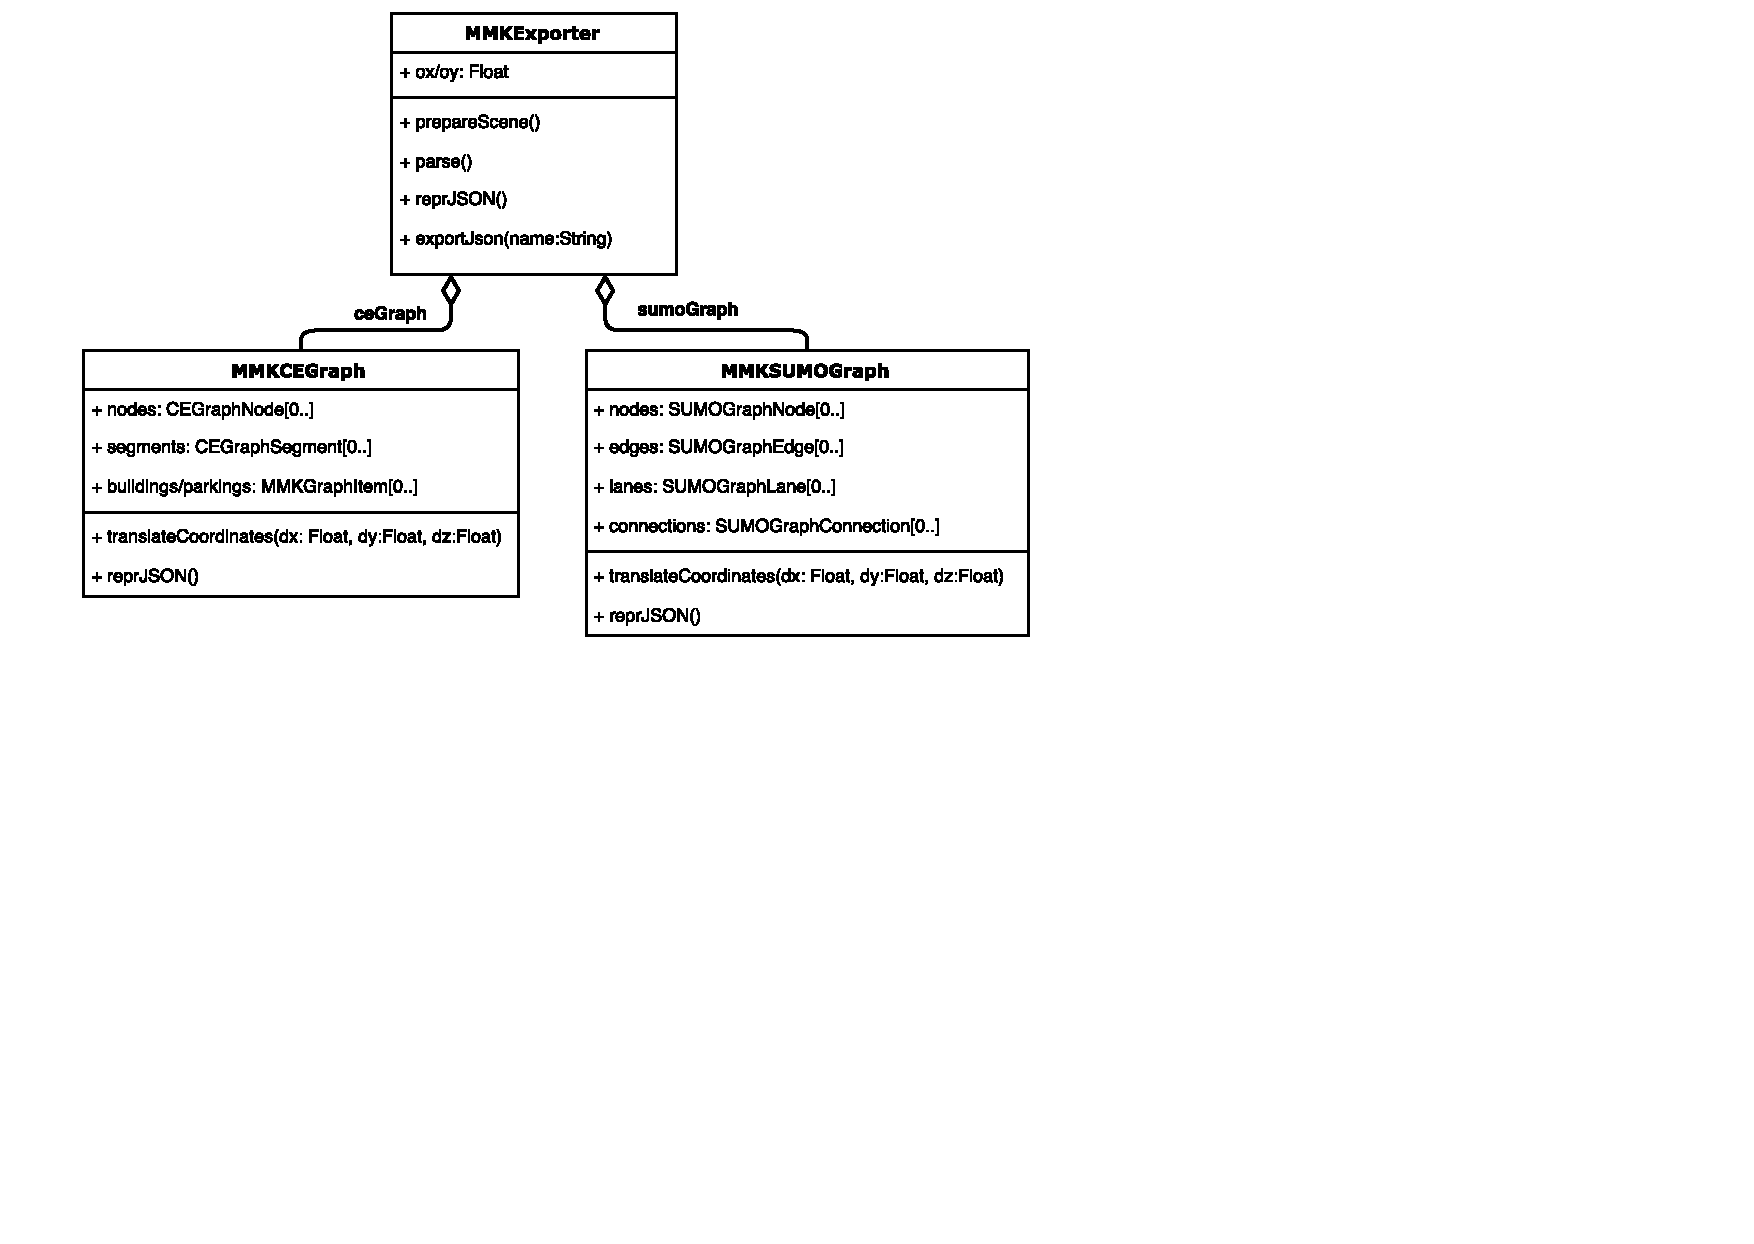
\includegraphics[width=0.7\textwidth]{figures/ce-overview-uml}
	\label{fig:ce-overview-uml}
	\caption{}
\end{figure}

\subsection{Additional Information from SUMO}
Synchronisation between CE and SUMO - lanes, node search, offset search (location kurzweg)
\begin{figure}[htb]
	\centering
	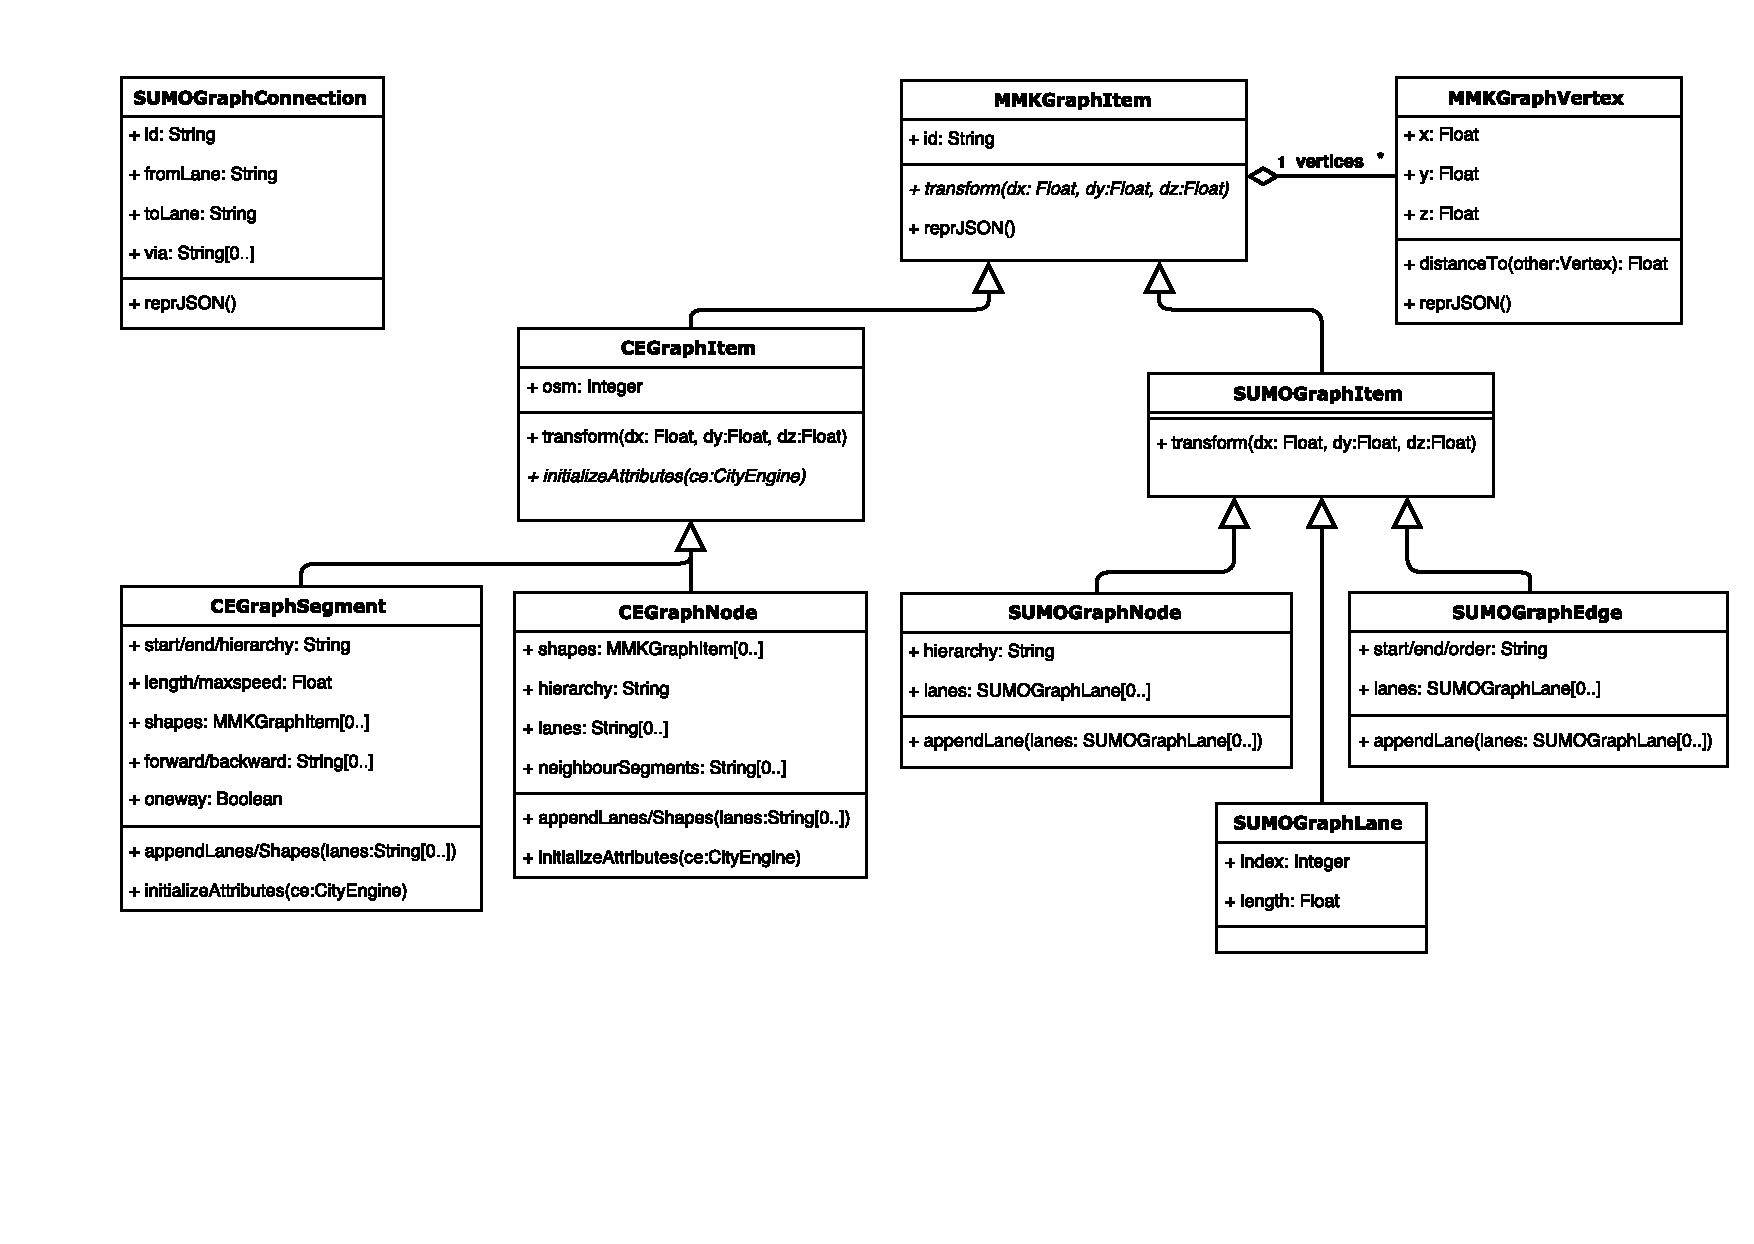
\includegraphics[width=0.9\textwidth]{figures/ce-uml}
	\label{fig:ce-uml}
	\caption{}
\end{figure}

\section{Format Description}
\label{sec:format}
As already introduced, we adopt a JSON format to hold the contents of the semantic description of a road network. In the following we discuss its advantages and disadvantages, as well as present all essential key value pairs used in the format.

In the beginning of this project, there was an idea to export the street network in OpenDRIVE format which was mentioned in the Chapter \ref{ch:background} in connection to other related work. Although OpenDRIVE allows a precise description of a road network and moreover, it is open-source and can be freely adopted, we withdraw from using it because of synchronisation reasons. More precisely, the data saved in OSM format has to be interpolated\cite{shi2011automatic}, which would introduce once again another desynchronisation between the network built by CE and the SUMO simulation. If this happens, the interpolated lanes in a hypothetical OpenDRIVE format would not coincide with the lane information generated by SUMO. Therefore, SUMO may not be able to be integrated as a simulation environment. Additionally, a JSON format, which we have chosen, has proven to be more human readable and easier to parse. Moreover, there exist a Unity module (Chapter \ref{ch:background}) which allows easier parsing. A JSON-based format gives us the opportunity to simultaneously provide a thorough description of a certain road network but also adopt and combine other data without breaking their coexistence. 

In Listing \ref{lis:format-1} one can see a general overview of the used JSON format. Firstly, we define the \texttt{author}, \texttt{date} of the export and the name of the \texttt{project}. These can be also changed in the script to arbitrary values. The more crucial parts of the export are \texttt{nodes} and \texttt{segments}. Obviously, each of these arrays hold all of the nodes, respectively segments in the CE scene. Previously, in the Research project by Max Mauerer, next to these values, there were also the number of all elements. We have chosen to eliminate these values since every parsing process can count the elements in each array. Next, the JSON export contains the \texttt{offsets} of CE and SUMO which was applied to each vertex coordinates in order to compose one coherent scene. Then, we have the \texttt{connections} array which holds the information about all possible connections between lanes. This helps us to build a navigation system in next chapter. Lastly, \texttt{sceneObjects} hold vertex information about other other objects in the scene which have no direct connection to the road network, \emph{e.g.} buildings, parkings.\\

	\begin{lstlisting}[language=json,firstnumber=1,caption={General overview of the used JSON format for description of road networks.},label={lis:format-1}]
{
    "author": "TUM - MMK",
    "connections": [(*@$\dots$@*)],
    "date": "2017-11-13",
    "lanes": [(*@$\dots$@*)],
    "nodes": [(*@$\dots$@*)],
    "offsets": {(*@$\dots$@*)},
    "project": "cityengine-mmk",
    "sceneObjects": {(*@$\dots$@*)},
    "segments": [(*@$\dots$@*)]
}
	\end{lstlisting}

A sample \texttt{node} value can be seen in Listing \ref{lis:format-node}. Firstly, we define its hierarchy which is defined by SUMO and can be one of these values: \emph{unknown}, \emph{priority} or \emph{traffic\_light} depending on the kind of node. Secondly, each node holds information about every lane which is part of it. Next, we find two id values in the export: \emph{id} is the \texttt{OID} value generated by CE and \emph{osm} is obviously its OSM ID. Each node's neighbouring segments are also referenced in the export by their id values. A node can have zero or more shapes which properties can be found in the \texttt{shapes} array. Additionally, each shape has again two kind of id values (identical to the node's ids). Finally, the coordinates of each node are kept in the \texttt{vertices} key.\\
 	
    \begin{scriptsize}
        \begin{lstlisting}[language=json,firstnumber=1,caption={General overview of the node key in the JSON exportformat.},label={lis:format-node}]
(*@$\dots$@*)
"nodes": [
    {
        "hierarchy": "priority",
        "id": "40170885-31eb-11b2-8d80-00e8564141ba",
        "lanes": [
            ":21457467_0_0",
            (*@$\dots$@*)
        ],
        "neighbourSegments": [
            "46535ea4-31eb-11b2-8d80-00e8564141ba",
            (*@$\dots$@*)
        ],
        "osm": 21457467,
        "shapes": [
            {
                    "id": "40170885-31eb-11b2-8d80-00e8564141ba:0",
                    "osm": 21457467,
                    "vertices": [
                        {
                            "x": 227.979736328125,
                            "y": -0.0,
                            "z": 109.73065185546875
                        },(*@$\dots$@*)
                    ]
            }
        ],
        "vertices": [
                {
                    "x": 232.09375,
                    "y": -0.0,
                    "z": 106.30369567871094
                }
            ]
        }
        (*@$\dots$@*)
]
(*@$\dots$@*)
	   \end{lstlisting}
    \end{scriptsize}
    
Similarly to a node, each segment has two id values (OID and OSM ID) as well as analogous \texttt{shapes} key. The \texttt{hierarchy} key provides the type of road defined by OSM and each possible value has been described in Chapter \ref{ch:background}. Next, segments define in their \texttt{lanes} key the direction of each lane (\texttt{forward} or \texttt{backward}). There are some self-explanatory attributes which are specific to segments such as \texttt{maxspeed}, \texttt{oneway}, \texttt{length}. Additionally, each segment holds a reference to its \texttt{start} and \texttt{end} node. Lastly, there is a \texttt{vertices} array holding a list of 3D polygon points which describe the overall shape of the segment.\\

\begin{scriptsize}
        \begin{lstlisting}[language=json,firstnumber=1,caption={General overview of the segments key in the JSON export format.},label={lis:format-lanes}]
(*@$\dots$@*)
"segments": [
    {
        "end": "4545af7a-31eb-11b2-8d80-00e8564141ba",
        "hierarchy": "tertiary",
        "id": "4545fc94-31eb-11b2-8d80-00e8564141ba",
        "lanes": {
            "backward": [
                "-392069506#0_0"
            ],
            "forward": [
                "392069506#0_0"
            ]
        },
        "length": 27.097801453973258,
        "maxspeed": "50",
        "oneway": false,
        "osm": 392069506,
        "shapes": [(*@$\dots$@*)],
        "start": "43422a00-31eb-11b2-8d80-00e8564141ba",
        "vertices": [(*@$\dots$@*)]
    }
]           
(*@$\dots$@*)
	   \end{lstlisting}
    \end{scriptsize}

Lanes objects are straightforward to describe. They posses an \texttt{id} field where their SUMO generated id is saved. Additionally, they have an index, length and a list of vertices describing their shape.\\
 
\begin{scriptsize}
        \begin{lstlisting}[language=json,firstnumber=1,caption={General overview of the lanes key in the JSON export format.},label={lis:format-node}]
(*@$\dots$@*)
"lanes": [
        {
            "id": ":315667013_8_0",
            "index": "0",
            "length": "7.88",
            "vertices": [
                {
                    "x": 34.27750000000003,
                    "y": 0.0,
                    "z": -110.02389160156247
                },(*@$\dots$@*)
            ]
        }
    ]
(*@$\dots$@*)
	   \end{lstlisting}
    \end{scriptsize}
    
Next, we take under consideration the connections objects. The only information they hold is that there is a connection between two lanes (\texttt{fromLane} to \texttt{toLane}). Since, two lanes might be connected through intermediate links, these links are noted in the \texttt{via} array.\\
    
    \begin{scriptsize}
        \begin{lstlisting}[language=json,firstnumber=1,caption={General overview of the connection key in the JSON export format.},label={lis:format-node}]
(*@$\dots$@*)
"connections": [
        {
            "fromLane": "-155040996_0",
            "id": 0,
            "toLane": "392103894#1_0",
            "via": [
                ":4972221472_0_0"
            ]
        }, (*@$\dots$@*)
    ]
(*@$\dots$@*)
	   \end{lstlisting}
    \end{scriptsize}
    
The scene objects are defined as shapes and have all of their properties as described above. Finally, we consider the \texttt{offsets} key which gives the translation parameters applied to every object from CE and SUMO in order to have the same coordinate system. \\

    \begin{scriptsize}
        \begin{lstlisting}[language=json,firstnumber=1,caption={General overview of the offsets key in the JSON export format.},label={lis:format-node}]
(*@$\dots$@*)
"offsets": {
        "ce": {
            "x": -690985,
            "z": 5336220
        },
        "sumo": {
            "x": 605.7575,
            "z": 595.5761083984376
        }
    },
(*@$\dots$@*)
	   \end{lstlisting}
    \end{scriptsize}
    
To summarise, the resulting export file with all of its features described in this section holds all of the necessary information about a given urban network. In the next section we discuss how it is imported in Unity.

\section{Unity Import}

Implementation details - UML
\begin{figure}[htb]
	\centering
	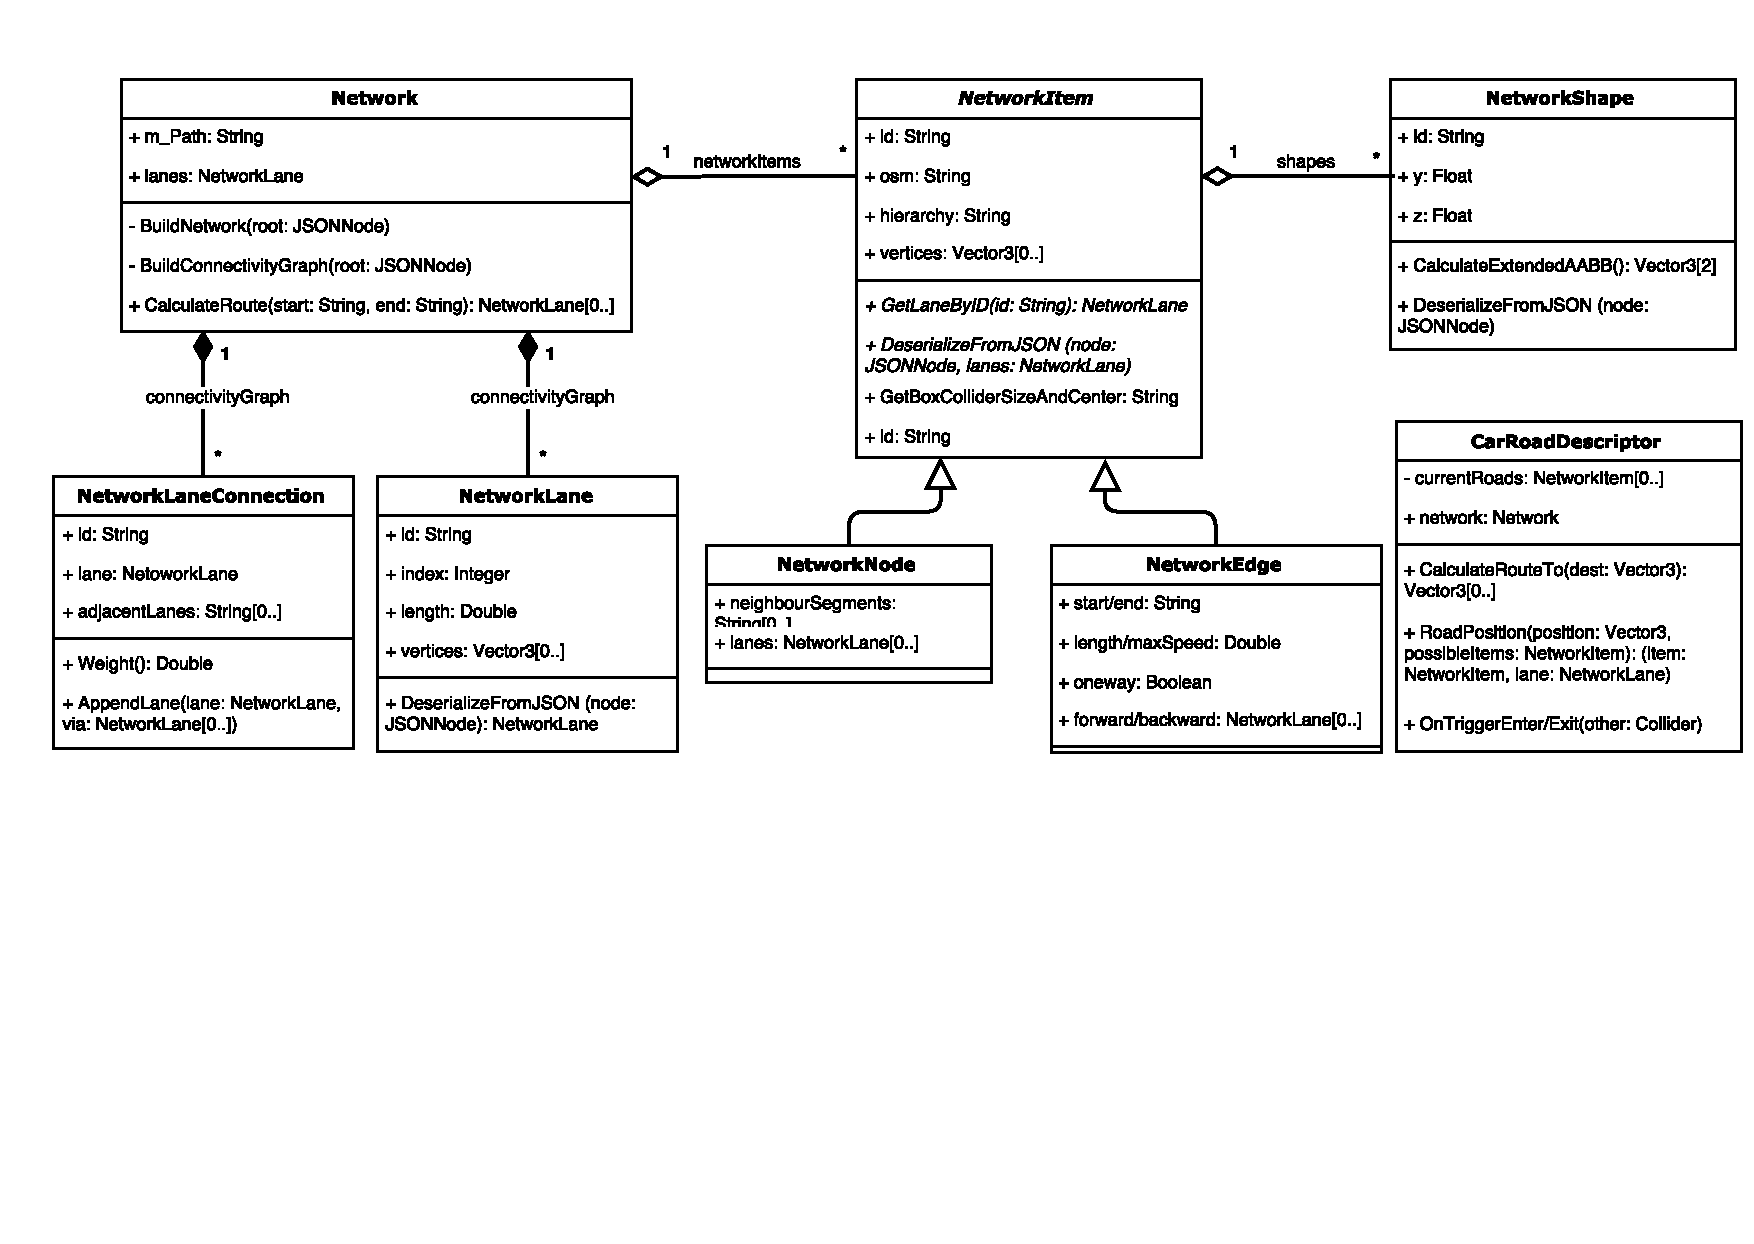
\includegraphics[width=0.9\textwidth]{figures/unity-uml}
	\label{fig:ce-overview-uml}
	\caption{}
\end{figure}

\chapter{Car Routing Algorithm}
\label{ch:gps}

\section{Overview}
\section{Dijkstra Algorithm}
\section{Implementation Details}
